\chapter*{Avant propos}
\thispagestyle{empty}
\section*{Histoire}
\setlength{\parindent}{20px}
L'histoire de la vision par ordinateur n'a pas pu enregistré une évolution considérable qu'après avoir introduire les techniques de l'intelligence artificielle.
Les recherches scientifiques ont profité de la quantité massive des données disponible pour développer des modèles mathématiques capables d'analyser ou de traiter un contenu numérique sans pour autant avoir recours aux méthodes classiques.
A titre d'exemple, on pourra juste imaginer le nombre de personnes nécessaire pour contrôler et approuver les publications sur une plate-forme comme Youtube (Chaque minute, 500 heures de vidéos sont mises en ligne). faisant le calcul pour le fun, 
il nous faut 225000 personnes pour les visualiser.

Les premiers algorithmes dans le domaine de l'intelligence artificielles reposent sur des données structurés qualitatives/quantitatives (alphanumérique) qui constituent des observations, des évènements des actions provenant plus ou moins du monde réel, cela renforce le doute qu'elle suivent un certain logique ou elle cachent des corrélations ou des phénomènes plus complexes. Donc le but est de chercher un modèle mathématique capable de faire la liaison entre les données et les résultats.
A ce stade, les statisticiens pourront revendiquer le droit que ce sont des problèmes d'ordre statistique, mais cette nuance disparaîtra au fur et à mesure que les objectives et les problèmes se diversifient.

Les réseaux de neurones n'ont pas seulement mis fin à ce débat mais ils ont encore poussé les limites de IA pour enfin parler de l'apprentissage automatique.
En laissant à côté les définitions, le réel apport de cette technologie par rapport au machine learning classique est que le choix des variables pertinents qui vont influer sur le résultat ou la prédiction ne va plus se faire par le "data-scientist" mais plutôt par la machine. Cette étape appelée feature-selection donne des résultats plus prometteuses d'une part, et d'autres part élargie le domaine d'applications. En effet, on n'est plus sous le contrainte d'étudier préalablement l'influence des variables pour y arriver au meilleur modèle. En d'autres termes le nombre des variables ne compte plus parmi les obstacles. l'autre aspect des réseaux de neurones est qu'ils permettent aux variables de s'interférer entre eux, plutôt d'affecter un poids à chaque variable dans les approches simplistes.

Jusqu'au là, les frontières se cernent autour des données structurées. il fallait trouver le moyen de représenter/codifier/métamorphiser les données non-structurées (images, vidéos, musique, ..) pour les faire "avaler" à nos fameux réseaux de neurones.

Nous y voici dans le Deep learning, dans les réseaux de neurones à convolutions. Cette technologie a gardé l'architecture des réseaux de neurones tel que  telle, et a ajouté un traitement/transformation sous forme de couches dites à convolution. Avec cette réadaptation, le réseau devient capable d'extraire les informations susceptibles d'être des caractéristiques pour les employer par la suite comme "features" d'un exemple. 
\vspace{1.5cm}
\begin{figure}[H]
\centering
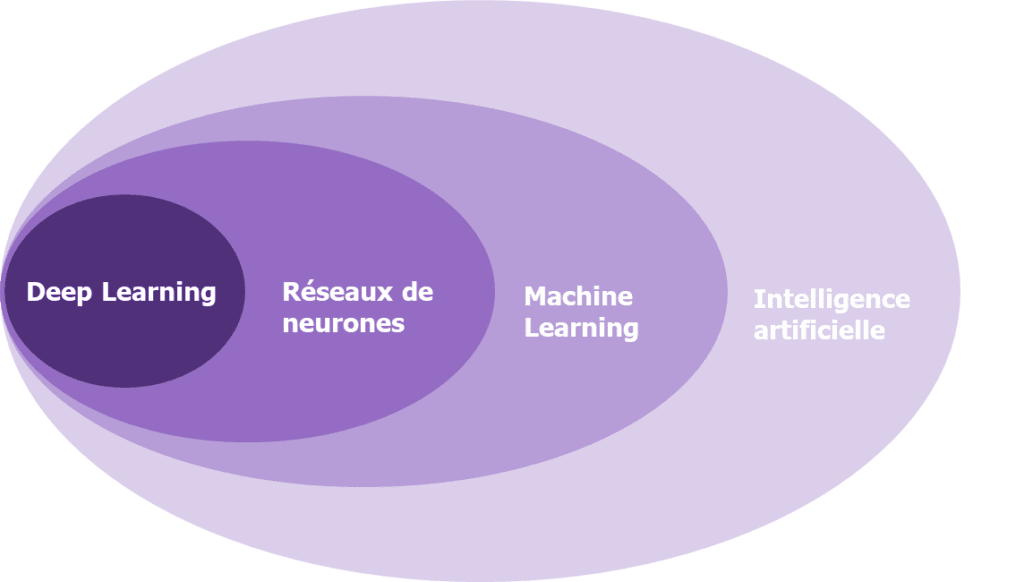
\includegraphics[width=12cm]{figures/AP/image-1-1.png}
\caption{Domaine de l'intelligence artificielle}
\end{figure}
